%----------------------------------------------------------------------------------------
%	PACKAGES AND OTHER DOCUMENT CONFIGURATIONS
%----------------------------------------------------------------------------------------
\documentclass[paper=a4, fontsize=11pt]{scrartcl} % A4 paper and 11pt font size
\usepackage[T1]{fontenc} % Use 8-bit encoding that has 256 glyphs
\usepackage{fourier} % Use the Adobe Utopia font for the document - comment this line to return to the LaTeX default
\usepackage[english]{babel} % English language/hyphenation
\usepackage{amsmath,amsfonts,amsthm} % Math packages
\usepackage{lipsum} % Used for inserting dummy 'Lorem ipsum' text into the template
\usepackage{sectsty} % Allows customizing section commands
\allsectionsfont{\centering \normalfont\scshape} % Make all sections centered, the default font and small caps
\usepackage{fancyhdr} % Custom headers and footers
\usepackage{amsmath}
\usepackage{graphics}
\usepackage{graphicx}

\pagestyle{fancyplain} % Makes all pages in the document conform to the custom headers and footers
\fancyhead{} % No page header - if you want one, create it in the same way as the footers below
\fancyfoot[L]{} % Empty left footer
\fancyfoot[C]{} % Empty center footer
\fancyfoot[R]{\thepage} % Page numbering for right footer
\renewcommand{\headrulewidth}{0pt} % Remove header underlines
\renewcommand{\footrulewidth}{0pt} % Remove footer underlines
\setlength{\headheight}{13.6pt} % Customize the height of the header

\numberwithin{equation}{section} % Number equations within sections (i.e. 1.1, 1.2, 2.1, 2.2 instead of 1, 2, 3, 4)
\numberwithin{figure}{section} % Number figures within sections (i.e. 1.1, 1.2, 2.1, 2.2 instead of 1, 2, 3, 4)
\numberwithin{table}{section} % Number tables within sections (i.e. 1.1, 1.2, 2.1, 2.2 instead of 1, 2, 3, 4)

\setlength\parindent{0pt} % Removes all indentation from paragraphs - comment this line for an assignment with lots of text

%----------------------------------------------------------------------------------------
%	TITLE SECTION
%----------------------------------------------------------------------------------------

\newcommand{\horrule}[1]{\rule{\linewidth}{#1}} % Create horizontal rule command with 1 argument of height

\title{	
\normalfont \normalsize 
\horrule{0.5pt} \\[0.4cm] % Thin top horizontal rule
\huge CS 760 Homework 5:\\ % The assignment title
\horrule{2pt} \\[0.5cm] % Thick bottom horizontal rule
}

\author{Qihong Lu} % Your name
\date{\normalsize\today} % Today's date or a custom date

\begin{document}

\maketitle % Print the title

\section*{Question1}
\textbf{
Show a neural network that represents the logical function $\mathbf{y = (x1 \land x2) \lor (x3 \land x4)}$. Specifically, show the network topology, weights and biases. You should assume that hidden and output units use sigmoid output functions, and an output-unit activation of 0.5 or greater represents a true prediction for y.\\ 
}

The network architecture is shown below. The weights are denoted in black. $X_i$ are the input units. $h_i$ are the hidden units. $b_i$ are the bias units. Finally, there is a single output unit. 

\begin{center}
	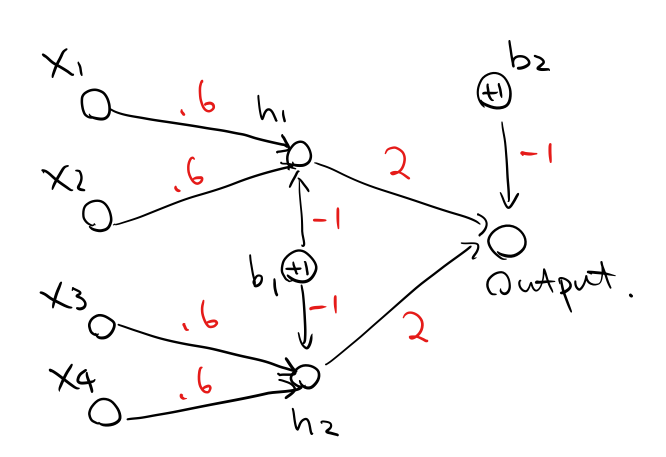
\includegraphics[scale=.4]{pics/hw5-1.png}
\end{center}


The unit h1 is representing an AND function over X1 and X2. 
Similarly, the unit h2 is representing an AND function over X3 and X4. Finally, the output unit represents an OR function over h1 and h2. 

\newpage
\section*{Question2}
\textbf{Consider the concept class C in which each concept is an interval on the line of real numbers. Each training instance is represented by a single real-valued feature x, and a binary class label \boldmath$y \in \{0, 1\}$. A learned concept is represented by an interval [a, a + b] where a is real value and b is a positive real value, and the concept predicts y=1 for values of x in the interval, and y=0 otherwise. Show that C is PAC learnable.}




\newpage
\section*{Question3}
\textbf{Consider the concept class that consists of disjunctions of exactly two literals where each literal is a feature or its negation, and at most one literal can be negated. Suppose that the number of features n = 3. Show what the Halving algorithm would do with the following two training instances in an on-line setting. Specifically, show the initial version space, the prediction made by the Halving algorithm for each instance, and the resulting version space after receiving the label of each instance.}

\begin{center}
\begin{tabular}{ c c c c}
 x1 & x2 & x3 & y \\ 
 T & F & F & pos \\  
 F & T & T & neg \\  
\end{tabular}
\end{center}





\newpage
\section*{Question4}
\textbf{In this same setting, suppose the learner can pick the next training instance it will be given. That is, the learner can pick the feature vector part of the instance; the class label will be provided by the teacher. Which instance should it ask for next? Justify your answer.}




\newpage
\section*{Question5}
\textbf{How many mistakes will the Halving algorithm make for this concept class in the worst case? Justify your answer.}




\newpage
\section*{Question6}
\textbf{Given the initial Bayes net parameters and training set depicted below, show how the network parameters would be updated after one step of the EM procedure. The `?' symbol indicates that the value for the variable A is missing in a given training instance.}
\begin{center}
	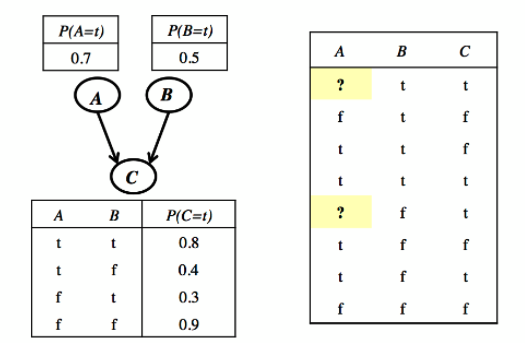
\includegraphics[scale=.5]{pics/hw5_6.png}
\end{center}



\newpage
\section*{Question7}
\textbf{Consider a learning task in which you are given n features and you want to use a feature selection method along with your learning algorithm. Specifically, suppose you are using forward selection along with k-fold cross validation to evaluate each feature set during the search process. Assume that there are r relevant features, and forward selection stops after selecting r features. Given a single training set, how many models are learned in the process of finding a feature subset of size r?}
\bigbreak

For forward selection, we begin with the null model (the model with no feature) and add one informative feature at each iteration, where the informativeness of a given feature is determined based on the cross-validated performance. 
\bigbreak
At the 1st iteration, there are n candidate features, I need to evaluate n models. \\
At the 2nd iteration, there are n-1 candidate features, I need to evaluate n-1 models. \\
......\\
At the r-th iteration, there are n-r candidate features, I need to evaluate n-r models. ($r \leq n$)
\bigbreak

Therefore, to chose r features, we need to evaluate $n (n-1) \cdots (n-r) $ models. \\

When evaluating each model, a k-folds cross validation is required. So in total, we need to fit $kn (n-1) \cdots (n-r)$ models. 

\newpage
\section*{Question8}
\textbf{Now suppose instead you are using backward elimination for the same task. Again, assume that the search process stops after selecting >r features and does not consider feature subsets smaller than this. Given a single training set, how many models are learned in the process of finding a feature subset of size r?}

For backward elimination, we begin with the full model (the model with all features) and remove the least informative feature at each iteration, where the informativeness of a given feature is determined based on the cross-validated performance. 
\bigbreak
1st iteration: there are n possible features can be removed, need to evaluate n models. \\
2nd iteration: there are n-1 possible features can be removed, need to evaluate n-1 models. \\
......\\
r-th iteration: there are n-r possible features can be removed, need to evaluate n-r models. ($r \leq n$)
\bigbreak

Therefore, to chose r features, we need to evaluate $n (n-1) \cdots (n-r) $ models. \\

When evaluating each model, a k-folds cross validation is required. So in total, we need to fit $kn (n-1) \cdots (n-r)$ models. 



\newpage
\section*{Question9}
\textbf{Consider the relational learning task defined below. List all of the literals that would be considered by FOIL algorithm on the first step of leaning a rule for the aunt(X, Y) relation. }
\begin{center}
	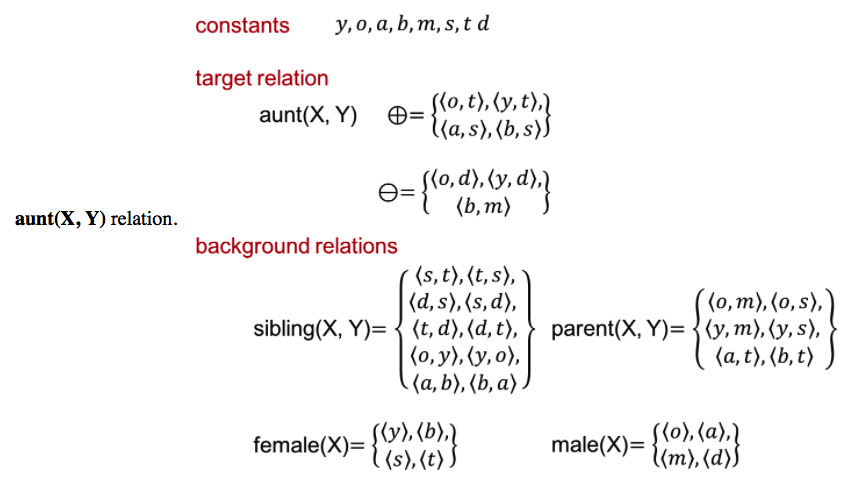
\includegraphics[scale=.4]{pics/hw5_9.png}
\end{center}



\newpage
\section*{Question10}
\textbf{Show the FOIL\_gain calculation when sibling(Y, Z) is considered as the first literal to be added to the first rule learning by FOIL. Also show the tuples that are involved in this calculation.}





\end{document}